\documentclass[10pt,twocolumn]{article}
% WS-077: rendered by make_paper.py from main.src.tex (do not edit main.tex; main.src.tex comes from md2tex.py).
\usepackage[margin=0.75in]{geometry}
\usepackage{graphicx,amssymb,hyperref}
\title{What a reward model can show depends on who stopped the episode: failure judges and monitors on a low-cost arm}
\author{Ravindu Somawansa\\Shisso Robotics}
\date{}
\begin{document}
\maketitle
\begin{abstract}
Watching a robot run only up to half the length of the task's longest run, elapsed time already separates failed from
successful runs with AUROC 0.851 within policy (CI 0.829--0.873) on 2,047 public SO-101 rollouts from 7 policies: failed runs
are slow, not timed out (only 8.7 \% reach the task's longest length). The dataset's stopping rule decides what a reward model
can show: where runs end at a time limit, elapsed time is the reward model to beat; where an operator stops them,
length is blind and a judge at rest works. Over the whole run, length gives 0.938 pooled and 0.942
within policy; two zero-shot reward models proposed as failure detectors score below it: Robometer-4B 0.818 pooled
(within policy pending) and TOPReward with an 8B video-language model 0.653 pooled, 0.661 within policy.
On 69 of our own operator-stopped rollouts length carries nothing (0.56), and TOPReward's
0.82 there is below what policy identity alone gives (0.87). A deterministic top-camera check at rest
makes no false positive; a robot-trained 27B judge separates every failure from every success (AUROC 1.00;
8 of 8 at 2 of 42 at a threshold chosen on the same episodes), and its base model does almost as well
given the same input; every mid-episode monitor we tested misses its bar. Report a length baseline, within policy, and
say who stopped the episodes.
\end{abstract}
\section{Introduction}
A reward model that scores robot rollouts is also a failure detector, and papers evaluate it as one. None of the
reward-model papers in our library reports how far plain episode length gets on the same data. We measure it on a
public SO-101 benchmark and on our own rollouts, with the analyses frozen before the numbers, and set every learned
judge and monitor we ran against it.

\section{Data and labels}
ArmnetBench v0.1 (SO-101, 8 tasks, 7 policies): 2,047 policy rollouts with a success or failure class
(515 successes, 1,532 failures); teleoperated episodes excluded. Our rollouts: 88 labelled bowls-task episodes
on one SO-101 and a Jetson Orin NX, and the 50-episode subset (42 successes, 8 failures) every monitor gate used. Labels
are the operator's, not blind to policy.

\section{The length baseline}
Pooled over policies, length gives 0.938 (CI 0.925--0.951); Robometer-4B, run zero-shot
as its authors ship it, 0.818 (CI 0.790--0.843; within policy pending its per-episode scores); TOPReward
(Qwen3-VL-8B, no training; the primary score, fixed in the protocol before any score, is the paper's success score, the sum
of its two standardised components) 0.653 pooled (CI 0.623--0.684) and 0.661
within policy (CI 0.631--0.692), below length by -0.31 to -0.25 (paired 95 \% CI). Its full-video
Yes/No component alone, descriptive: 0.678 within policy. Within each policy, length ranges 0.91--0.96, pair-weighted
0.942 (CI 0.927--0.956): it is not the policy identity (Fig. 1).



\begin{figure}[t]\centering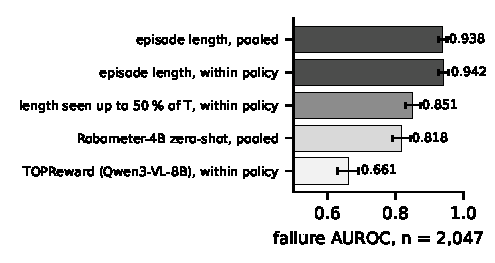
\includegraphics[width=\columnwidth]{fig/armnetbench.pdf}\caption{Failure AUROC on ArmnetBench (95 \% CIs): episode length vs two zero-shot reward models (Robometer-4B, TOPReward with Qwen3-VL-8B).}\end{figure}

\section{Is it the timeout?}
Only 8.7 \% of failures run to the task's longest episode. Observing length only up to half of that, when
88 \% of failures but 19 \% of successes are still running, gives 0.851 within policy
(CI 0.829--0.873; Fig. 2; TOPReward on frames up to the same cut: 0.667): failed rollouts are slow, not timed out. Both pre-registered readings hold: length is a
within-policy null, and it is more than the timeout. On our own operator-stopped rollouts the same baseline is at chance
(0.56 on 69; 0.52 on all 88). Neither reward model beats the policy-identity null there:
TOPReward 0.82 (CI 0.70--0.93) against 0.87 for policy identity alone, and
0.78 on the 50 episodes without TurboVLA (17 of the 25 failures in the
69 come from TurboVLA); Robometer 0.577 against 0.878 on 88. The baseline depends on how
episodes end, which is why it must be reported per dataset; what works on operator-stopped runs is the judge at rest (§5).



\begin{figure}[t]\centering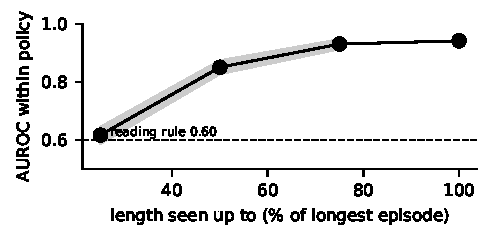
\includegraphics[width=\columnwidth]{fig/truncation.pdf}\caption{Length observed up to a fraction of the task's longest episode, AUROC within policy (band: 95 \% CI).}\end{figure}

\section{Judges and monitors on our rollouts}
\textbf{At rest.} A deterministic top-camera check (colour masks and geometry, no learning) is right on 94.3 \% of
judged episodes with 0 false positives (Wilson 0–13 %) and 5 false negatives. Given a 64-frame
two-view clip and NVIDIA's prompt, Flora-Rewarder-27B separates every failure from every success (AUROC 1.00, the
threshold-free number); at its gate's operating point, a score threshold chosen on these same 50 episodes, it flags
8 / 8 failures at 2 / 42 successes (Wilson on the false alarms 1–16 %) and passes its bar; its base
model Qwen3.5-27B gets 7 / 8 at 2 / 42 on the same input at its own in-sample threshold; a 9B model (0.75) and Gemini 3.8 Flash (0.96, one false alarm over the
bar) do not pass. The input format, not the robot fine-tune, decided the result.

\textbf{Mid-episode.} A Gemini sliding-window judge catches 0 / 8; the surprise of a separate world model
2 / 8 (AUROC 0.86, Wilson 7–59 %); latent drift 0 / 8. An action-conditioned risk head on
the world model's latent reached 0.93 in a first version that read elapsed time; the pre-registered second version,
without time or length, catches 3 / 8 at 5 / 42 (AUROC 0.79 vs 0.71 with shuffled
actions; Wilson 14–69 %), and its MLP variant 6 / 8 at 13 / 42: \textbf{no monitor meets the bar}
($\geq$ 5 / 8 at $\leq$ 1 / 20), and the first version's result is withdrawn (Fig. 3).



\begin{figure}[t]\centering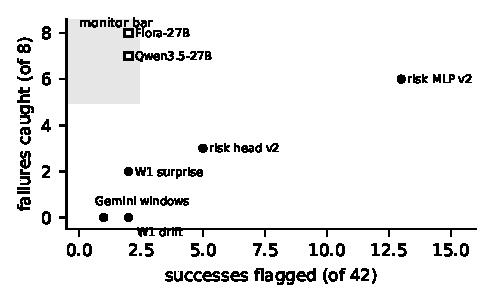
\includegraphics[width=\columnwidth]{fig/own_monitors.pdf}\caption{Fifty own rollouts: failures caught (of 8) vs successes flagged (of 42). Circles: mid-episode monitors; shaded: their bar ($\geq$ 5/8 at $\leq$ 1/20). Squares: judges at rest (one score per finished episode) at their in-sample G-flora operating point; the monitor bar does not apply to them.}\end{figure}

\section{Limitations}
Two task families (ArmnetBench's eight tasks, our bowls task); our labels are the operator's and not blind; the risk
head is trained and tested on the same 50 episodes (5-fold by episode: episodes do not leak, tasks and policies do);
Robometer under the within-policy and truncation analyses is pending its per-episode scores; TOPReward's prefix
count, frames per query and Yes/No wording are not given in its paper and are ours; the operating points of Flora,
Qwen3.5-27B and Gemini are chosen in-sample on the 50 episodes they are scored on (their AUROCs are not); 17 of
the 25 failures in our 69 rollouts are TurboVLA's, so on our set any score that reads the policy gets the
identity null for free; the timeout is
approximated by each task's longest episode.


\section*{References}
Robometer 2603.02115 · SARM 2509.25358 · TOPReward 2602.19313 · VLLR 2604.00055 · SARM2 2606.10305 · STDR 2606.31377 ·
No Free Checker 2609.09250 · FARM 2609.11445 · ReAP 2610.16309 · SAFE 2506.09937 · FAIL-Detect 2503.08558 ·
VLA-Corrector 2609.06508 · Spotter 2609.36808 · REMORA 2610.39125 · ArmnetBench 2607.24481 · SO-101 benchmark 2606.08881.
\end{document}
